\documentclass[12pt,peerreviewca, a4paper, onecolumn]{article}

\pagenumbering{gobble}

\title{\LARGE\textbf{Looking For Caresses with MiRo}\\\large For Social Robotics Course 2018/19}
\author{\large{Torielli Davide \quad Fusaro Fabio} \\
	\small EMARO - European Master on Advanced Robotics\\
	\small DIBRIS - Dip. Informatica, Bioingegneria, Robotica, Ing. Dei Sistemi\\
	\small Universit\`{a} Degli Studi Di Genova, \today}

\usepackage{hyperref}
\hypersetup{colorlinks=true, linkcolor=blue}
\usepackage[a4paper,left=40px,right=40px,top=50px,bottom=10px,
includefoot,heightrounded]{geometry}
\usepackage{amsmath}
\usepackage{relsize}
\usepackage{amssymb}
\usepackage{graphicx}
\graphicspath{ {./images/} }
\usepackage{caption}
\usepackage{floatrow}
\usepackage{titlesec}
\titleformat{\section}[block]{\large\bfseries}{\thesection}{4mm}{}

\titleformat{\subsection}[block]{\normalsize\bfseries}{\thesubsection}{2mm}{}

\begin{document}
	\maketitle
	
	\section{Introduction}
	MiRo from Consequential Robotics is a bio-inspired robot. It has different sensors to interact with the enviroment: cameras, cliff sensors, light sensor, sonar, microphone.\\
	In this project, MiRo behave as companion, standing on the desk while the user is working (for example, at pc). We exploit joints and sensors to make the robot interact with the user, and make MiRo act like a pet should do: making noise, show sleepiness, wag tail if happy, and so on.	
	
	Like a real pet, MiRo wants attentions from the user. We have implemented this thing in a simply way. A \textbf{loneliness} value ranges from 0 to 100. When it is low, MiRo more probably will wake up, because it feels lonely and he wants caresses. While the interaction is going on, and the user caresses  MiRo, this level goes down. The more the level is low, the more MiRo will probably goes to sleep.
	
	\section{The Code}
	\begin{center}
		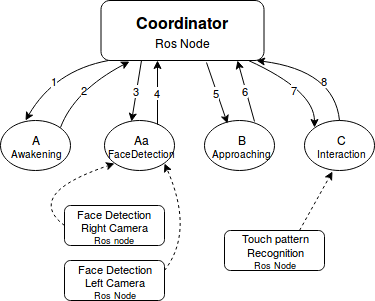
\includegraphics[scale=0.5]{diagram}
	\end{center}
	{\small The diagram on the code structure: straight line with numbers resprent execution flow. After step 8 the cycle begin again from step 1. Dotted line represent data exchanged through ros publish-subscribe method.  The communications with the robot (again with ros topics) to receive sensor data and send platform command are not shown}\\

    \newpage
	\noindent The \textbf{coordinator} is a ROS node responsible to call different classes related to the 4 different phases: Awakening (\ref{subsec:a}); Face Recognition (\ref{subsec:aa}); Approaching (\ref{subsec:b}); Interaction (\ref{subsec:c}).
	\subsection{Task A: Awakening Phase}
	\label{subsec:a}
	In task A, MiRo is sleeping. The task sends through ROS topic commands to shown this. This results in MiRo with close eyelids and head down. While sleeping, \textbf{loneliness} value increases, until MiRo woke up or is is touched by user.
	\subsection{Task Aa: Face Recognition Phase}	\label{subsec:aa}
	Now MiRo looks for user face. To do this, we rely on the \textit{face detector} node. This node (from open-cv-apps package) is subscribed to the topic where left and right cameras send image flow. Then, it publish face detection infos on another topic. We read from this topic if a face is detected or not.
	If MiRo does not see a face with neither cameras, it turns on z axis. If it see a face with one cameras, it turn a bit slower clockwise or counter-clockwise to catch the face with both cameras, and at this point it stops turning. When MiRo see the face with both cameras for 3 consecutevely seconds, the task finished.
	\subsection{Task B: Approaching Phase}	\label{subsec:b}
	MiRo gets near to the user using the sonar on his muzzle. The user should put the hand toward MiRo muzzle, to start interaction with him. If the sonar detect something (i.e., the hand) sufficently near, MiRo stops and next phase starts.
	\subsection{Task C: Interaction Phase} 	\label{subsec:c} 
	The user can choose to interact or not with MiRo. If he rubs him on the body, the \textbf{loneliness} value will decrease. Meanwhile, MiRo will act like real pet: the more is rubbed the more he shown his happiness waging the tail, moving the ears, and making "mammal" sounds.\\
	If the user does not want to interact any more, he must pat MiRo on head, and he will immediately go to sleep, but with a higher value of \textbf{loneliness}.\\
	To understand the touches, we use a node implemented by others ().
	The chances to make MiRo go to sleep increase if \textbf{loneliness} value decrease. After the interaction phase, the Sleeping phase is recall and the cycle repeats. 
	
	\section{Further Works}
	The more critical phase is the interaction one. The sensors of MiRo are really simple (binary ones) and the one on the head not so intuitive and easy to use. Also, they are positioned on particular point, and not spread on the whole body. For this, the pattern recognition algorithm is difficult to use. To solve the problem, if the user wants to interact with MiRo he has to rub him on body, and, if not, touch him on head. This to avoid confusion in detecting the pattern. A further work can focuses on this particular problem.\\
	Also the face recognition can me improved, helping in someway the task, for example, moving and not only turning or exploit the other joint of the neck (pitch and yaw).\\
	Another work could be done in improving the interaction, exploiting, for example, also the microphones on MiRo ears.
 
	 
		

	
\end{document}